%===============================================================================
% IronClaw conference paper (IEEE conference format)
% Condensed from the undergraduate thesis report and defense slides.
%
% Build:  make paper
% Manual: TEXINPUTS="./fontmetrics/tex//:" TFMFONTS="./fontmetrics/fonts/tfm//:" \
%           pdflatex paper && bibtex paper && pdflatex paper && pdflatex paper
%
% Note: fontmetrics/ contains Times/Helvetica TFM metrics and binhex.tex.
% IEEEtran samples Times metrics at class load, and newtxtext needs binhex;
% neither is installed system-wide on this machine, so the local copies must
% stay on the TeX search path (the env vars above do that).
%===============================================================================
\documentclass[conference]{IEEEtran}

% Times-like text and math fonts (IEEE style); newtx is used because the
% classic psnfss Times metrics are not installed on this system.
\usepackage{newtxtext,newtxmath}

\usepackage{cite}
\usepackage{amsmath}
\usepackage{graphicx}
\usepackage{booktabs}
\usepackage{array}
\usepackage{multirow}
\usepackage{xcolor}
\usepackage{url}
\usepackage[hidelinks]{hyperref}

\newcommand{\toolname}{IronClaw}

\hyphenation{Fire-cracker micro-VM}

\begin{document}

\title{IronClaw: Dynamic Tool Synthesis and Secure MicroVM\\Isolation for
Autonomous LLM Agents}

\author{\IEEEauthorblockN{Suryavir Kapur and Vijay Kumar Balakrishan}
\IEEEauthorblockA{Department of Computer Science \& Information Systems\\
Birla Institute of Technology and Science Pilani\\
Email: f20220293@dubai.bits-pilani.ac.in}
}

\maketitle

%===============================================================================
\begin{abstract}
Large Language Model (LLM) agents increasingly execute complex multi-step
workflows. When no purpose-built capability exists, an agent can either author
the required logic inline on every request or synthesize a task-specific tool
once and reuse it. Reuse promises efficiency gains, but executing synthesized
code in an ordinary process creates significant security risk. This paper
presents \toolname, an autonomous-agent platform that combines dynamic tool
synthesis with strictly isolated Firecracker microVMs. A trusted host daemon
manages agent policy, context, and lifecycle, while an ephemeral guest runtime
executes generated code behind a hardware-virtualization boundary, reachable
only over an authenticated protobuf/vsock channel. We evaluate the two
resulting claims independently. On the utility side, across SQL, log-parser,
and repository-compliance domains, registering and reusing synthesized tools
reduced billed input tokens by 53.4\%, 61.4\%, and 53.6\% on repetitive
workloads relative to inline authoring, with 100\% answer correctness in both
conditions; on mixed workloads with only three-of-six reuse, synthesis was
net-negative (+19.0\% and +64.7\% input tokens). On the security side, all
five host-resource attacks succeeded under ordinary process execution and none
succeeded inside Firecracker; containment cost a 6.08\,s median cold start, a
6.62\,s median recovery, and 72{,}672\,KiB host resident memory for a
512\,MiB guest, while warm dispatch over an existing session cost only
1.74\,ms. Dynamic synthesis therefore pays off exactly when reuse is expected,
and microVM isolation is practical today for long-lived agent sessions;
per-request isolation awaits snapshot restore.
\end{abstract}

\begin{IEEEkeywords}
autonomous agents, large language models, dynamic tool synthesis, Firecracker,
microVM, sandboxing, isolation, vsock
\end{IEEEkeywords}

%===============================================================================
\section{Introduction}
LLM-based autonomous agents are being applied to long-horizon tasks in software
engineering, data management, document processing, and process automation.
Most deployed agents operate with a \emph{static registry} of predefined tools
chosen by their developer before the task begins. Static registries simplify
auditing and permissioning, but they cannot cover the intermediate parsers,
converters, checks, and integrations that open-ended tasks routinely demand.

\emph{Dynamic tool synthesis} (DTS) removes this limitation: the agent writes a
small program, executes it, observes the result, and registers it as a reusable
capability. This changes the security model. Generated code can contain
destructive operations, command-injection payloads, resource-exhaustion loops,
or deliberate host escapes, whether by model error or prompt injection.
Sandboxing only the process that hosts the agent is therefore insufficient:
agent-generated code must be treated as adversarial regardless of how benign
the user's request appears.

\toolname{} addresses this joint utility/security problem by pairing DTS with
Firecracker microVM isolation. A trusted host daemon owns the agent loop,
policy, memory, LLM access, and VM lifecycle; an intentionally small,
ephemeral guest runtime executes untrusted tool code inside a
hardware-virtualization boundary and returns only bounded, structured results
over an authenticated vsock channel. The design lets us measure both sides of
the trade-off with matched baselines, guided by two research questions:

\begin{itemize}
\item \textbf{RQ1 (Utility).} On repeated tasks with no purpose-built tool,
does dynamic tool synthesis reduce model interaction steps and token
consumption relative to authoring the logic inline, without reducing
correctness?
\item \textbf{RQ2 (Security/Systems).} What containment capability and
performance overhead does Firecracker microVM isolation provide compared with
process-level execution of agent-generated code?
\end{itemize}

\noindent Our contributions are:
\begin{enumerate}
\item \textbf{An architecture} that integrates dynamic tool synthesis with
ephemeral microVM execution behind a strict host/guest boundary, implemented as
a Rust workspace (host daemon, guest runtime, shared protocol/transport
crates) with process, container, and microVM sandbox backends.
\item \textbf{A utility evaluation} across three domains (SQL synthesis,
legacy-log parsing, repository compliance) showing that reuse of synthesized
tools cuts billed input tokens by 53.4--61.4\% and model steps by up to 46.4\%
on repetitive workloads while preserving 100\% correctness---and that the same
mechanism is net-negative when reuse is sparse.
\item \textbf{A security and performance evaluation} showing 0/5 successful
host-resource attacks inside Firecracker versus 5/5 under process execution,
with measured costs: 6.08\,s median cold start, 6.62\,s median recovery,
72{,}672\,KiB host resident memory, and 1.74\,ms warm dispatch.
\end{enumerate}

Section~\ref{sec:background} reviews background and related work.
Section~\ref{sec:design} presents the \toolname{} architecture.
Section~\ref{sec:methodology} describes the evaluation methodology.
Sections~\ref{sec:utility} and~\ref{sec:security} report the utility and
security/performance results. Section~\ref{sec:discussion} discusses
limitations, and Section~\ref{sec:conclusion} concludes.

%===============================================================================
\section{Background and Related Work}
\label{sec:background}

\subsection{LLM Agents and Tool Use}
LLM agents extend language models with external tool calls, task state, and
multi-step planning, delegating exact computation and program execution to
deterministic systems. ReAct showed that interleaving reasoning traces with
actions improves interactive task solving~\cite{yao2023react}; Toolformer
showed that models can learn when external API calls are
useful~\cite{schick2023toolformer}; Generative Agents demonstrated memory,
reflection, and planning loops~\cite{park2023generative}; and Voyager showed an
agent accumulating executable skills in an open-ended
environment~\cite{wang2023voyager}. Despite this progress, most deployed
agents still rely on static tool registries, which eases auditing but prevents
runtime capability creation. Benchmarks such as SWE-bench evaluate reasoning
over real repositories~\cite{swebench}; our evaluation instead targets the
tasks most likely to benefit from tool generation---parsing, checking,
transforming, and repeated verification.

\subsection{Dynamic Tool Synthesis}
DTS targets work whose required code cannot be predicted in advance:
converting unknown file formats, aggregating benchmark outputs, validating
configurations, or building domain-specific checks. The agent authors code,
runs it in an isolated environment, inspects the output, and then revises or
reuses the artifact. Our utility experiments quantify when this create-once,
reuse-many pattern is worth its creation cost.

\subsection{Isolation: Processes, Containers, VMs, MicroVMs}
Process isolation relies on the host OS memory and permission model: all
processes share the host kernel, so a kernel bug or misconfiguration can
escalate a process compromise into a host compromise. Containers add
namespaces, cgroups, and capabilities but still share the host kernel.
Virtual machines run a guest OS on virtualized hardware, so privileged
operations are mediated by a hypervisor, satisfying the classic VMM goals of
equivalence, resource control, and efficiency~\cite{popek1974formal}; Xen is a
canonical example~\cite{barham2003xen}. Hardware extensions (Intel VT-x/AMD-V)
run guest code directly on the CPU, trapping sensitive operations via VM exits
to the hypervisor~\cite{adams2006comparison,intel2025sdm}, while Extended Page
Tables enforce memory isolation between guests and host. MicroVMs keep the
hardware boundary but shrink the device model and management surface, making
them suitable for short-lived isolated workloads; Firecracker is a production
implementation designed for lightweight serverless
virtualization~\cite{agache2020firecracker}.
Figure~\ref{fig:isolation} summarizes this continuum. \toolname{} creates a
microVM per task session, runs the generated code, returns bounded output, and
discards the guest, preventing persistence and cross-tool contamination.

\begin{figure}[!t]
    \centering
    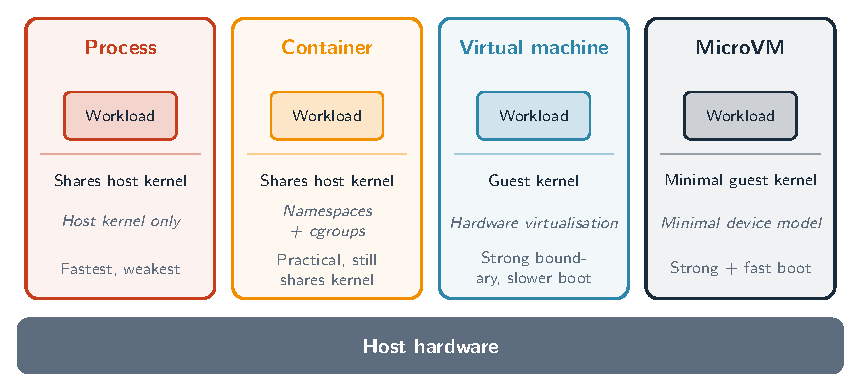
\includegraphics[width=\columnwidth]{Figures/fig_isolation_boundaries.pdf}
    \caption{Isolation continuum: process, container, VM, and microVM
    boundaries. Only VM-based boundaries remove the shared-kernel dependency.}
    \label{fig:isolation}
\end{figure}

%===============================================================================
\section{IronClaw Design}
\label{sec:design}

\subsection{Asymmetric Host/Guest Split}
\toolname{} is built around a strict split of trust
(Figure~\ref{fig:architecture}). The host daemon (\texttt{ironclawd}) is
trusted and stateful: it loads configuration, enforces policy, manages memory,
talks to LLM providers, and controls the microVM lifecycle. The guest runtime
(\texttt{irowclaw}) is untrusted and ephemeral: it accepts bounded execution
requests, runs them under local limits, returns structured results, and can be
destroyed at the end of a session. Because generated tools are untrusted, the
host never executes them; it packages the tool specification and code for the
guest.

\begin{figure}[!t]
    \centering
    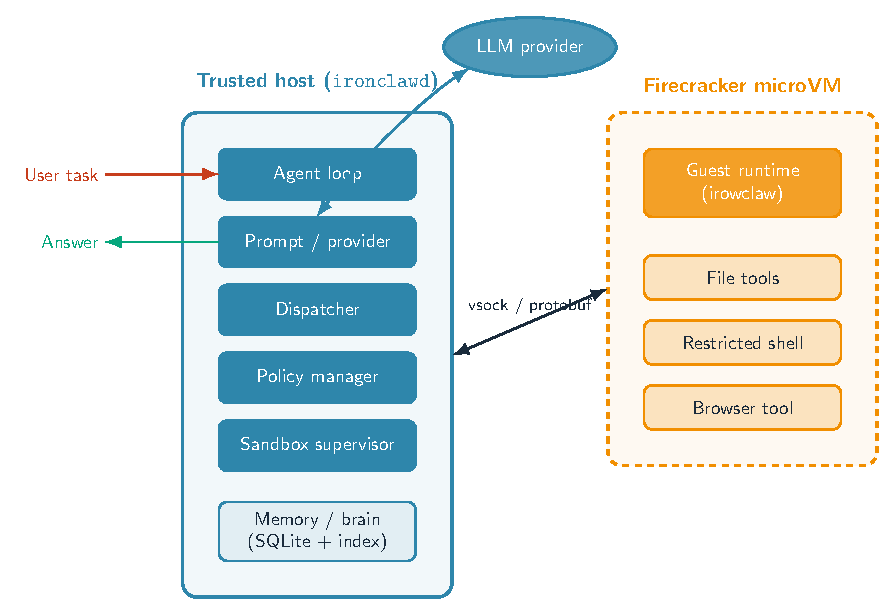
\includegraphics[width=\columnwidth]{Figures/fig_architecture.pdf}
    \caption{\toolname{} host/guest architecture. The trusted host daemon runs
    the agent loop and owns the sandbox lifecycle; generated tools execute
    inside a Firecracker microVM guest runtime.}
    \label{fig:architecture}
\end{figure}

Five host subsystems cooperate: (i) an \emph{agent loop} maintaining the
plan--act--observe cycle and deciding whether the next action is a fixed tool
call, a generated tool, or the final answer; (ii) a \emph{prompt/provider
layer} that builds prompts from task context, memory, tool results, and policy
reminders; (iii) a \emph{dispatcher} that normalizes model actions into typed
execution requests and routes them to local fixed tools or the guest; (iv) a
\emph{policy manager} that bounds filesystem access, network access, CPU time,
memory, output size, and allowed interpreters; and (v) a \emph{sandbox
supervisor} that creates, monitors, times out, and destroys guest runtimes.
The host also performs \emph{result triage}: guest responses are bounded,
decoded, tagged with status metadata, and summarized where necessary, so large
or malformed outputs cannot destabilize the next agent turn.

The guest runtime is deliberately minimal. It validates the request envelope
(request identifier, tool name, input payload, execution limits), materializes
the execution environment (input files, interpreter selection, local process
limits), and captures a structured response (exit status, stdout, stderr,
duration, error classification). It holds no secrets, credentials, or host
mounts: every byte needed for an execution is explicitly sent by the host, so a
payload inspecting the system sees only the minimal guest filesystem and the
inputs for that single run.

\subsection{Transport Boundary and Protocol}
Host and guest communicate over a controlled channel---an authenticated
protobuf envelope carried over Firecracker vsock (with in-memory and
child-process transports reused for testing). Each envelope carries
\texttt{user\_id}, \texttt{session\_id}, \texttt{msg\_id},
\texttt{timestamp\_ms}, and a \texttt{cap\_token}; the payload is a
\texttt{oneof} covering authentication (\texttt{AuthChallenge}/\texttt{AuthAck}),
agent control, user messages, tool calls/responses, file operations, and
scheduler events. Before execution, the host performs a capability handshake:
it sends a capability token and a tool allow-list, and the guest filters its
registry to only those tools. A request envelope is explicit rather than
shell-like: request id, tool name and type, code or command material,
serialized inputs, policy fields (timeout, memory, network mode, output limit),
and the expected result format. Responses mirror this structure with status,
exit code, duration, bounded stdout/stderr, and artifact metadata, letting the
host distinguish timeout, policy denial, runtime crash, and success instead of
treating every reply as plain text.

\subsection{Dynamic Execution Engine}
Tool generation and tool execution are kept separate: the model may propose
code, but the host decides eligibility and the guest confines the consequences.
The loop proceeds in six stages (Figure~\ref{fig:flow}): (1) the agent
identifies that no fixed tool suffices; (2) the model proposes a small tool
with purpose, inputs, and code; (3) the host validates the specification
against policy and rejects unsafe requests before guest execution; (4) the
guest runs the tool in the microVM and captures bounded outputs; (5) the host
classifies the result as success, tool error, policy error, timeout, or
infrastructure error; (6) the agent continues, revises the tool, or answers.

\begin{figure}[!t]
    \centering
    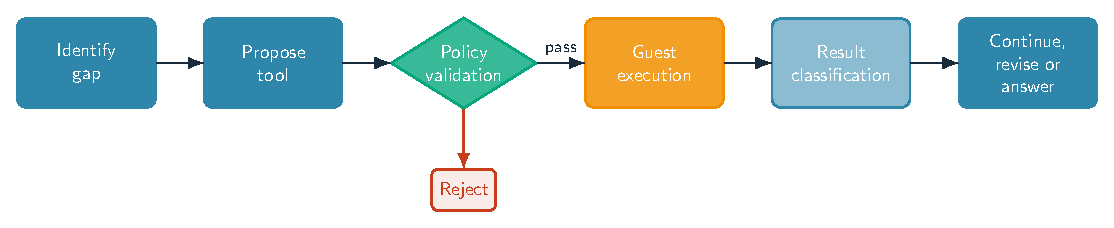
\includegraphics[width=\columnwidth]{Figures/fig_dynamic_tool_flow.pdf}
    \caption{Dynamic tool synthesis flow, showing the policy gate between tool
    proposal and guest execution.}
    \label{fig:flow}
\end{figure}

\subsection{Ephemeral Sandboxing and Failure Model}
Each session runs in an ephemeral microVM: allocate/resume the guest image,
establish vsock, send the request bundle, enforce host-side timeout and output
limits, receive and validate the response, copy out approved artifacts, then
destroy or reset guest state. This blocks cross-tool contamination, persistent
state abuse, and memory poisoning. Snapshot resume can reduce startup time but
must represent a clean base state, untainted by task-specific secrets or
previously generated tools. Every failure is classified (tool, policy,
timeout, transport), so the next agent step proceeds without exposing the host
to the failing execution.

\subsection{Implementation}
The system is a Rust workspace\footnote{Source:
\url{https://github.com/suryavirkapur/ironclaw}} separating the control plane
from the execution plane: \texttt{ironclawd} (host daemon, agent loop, sandbox
managers), \texttt{irowclaw} (guest runtime), \texttt{common} (configuration,
protobuf bindings, codec, transport traits, Firecracker abstractions),
\texttt{tools} (workspace-rooted file tools, restricted shell, headless
browser), \texttt{memory} (SQLite store with hybrid retrieval and redaction),
\texttt{security} (authentication, pairing, rate limiting), and
\texttt{channels}. The host supports \texttt{process}, \texttt{container}, and
\texttt{microvm} sandbox backends behind one manager abstraction, which lets
the same agent loop be evaluated under different containment strategies.
Firecracker guests boot a minimal kernel command line (\texttt{panic=1},
\texttt{pci=off}, \texttt{nomodules}, \texttt{root=/dev/vda},
\texttt{init=/init}); after \texttt{InstanceStart}, the host connects over the
vsock UDS, issues \texttt{CONNECT}, and wraps the stream in the same framed
transport used elsewhere. Guest-side safety checks (path rooting, shell
sub-string denylists, output caps, scheme validation) provide defense in depth
\emph{within} the guest---they complement, and do not replace, the
virtualization boundary.

%===============================================================================
\section{Evaluation Methodology}
\label{sec:methodology}

The evaluation measures utility, security, and systems performance
independently, with matched baselines for each hypothesis.

\subsection{Utility (H1): No Synthesis vs.\ Dynamic Synthesis}
Two scenarios share the same generic base capabilities and differ only in
whether the repeated artifact can be registered for reuse. \textbf{Scenario~A
(no synthesis):} the agent must author the required task logic inline for every
request. \textbf{Scenario~B (dynamic synthesis):} the same capabilities plus a
meta-tool and explicit policy to register the repeated logic once and reuse it.
The comparison holds data, requests, model, and generic capabilities constant.
The harness is a deterministic TypeScript experiment suite built on the Vercel
AI SDK and its \texttt{dynamicTool()} primitive~\cite{aisdk}; all conversations
use \texttt{deepseek-v4-pro}, a reasoning-enabled model~\cite{deepseek}.

Five experiments cover three domains:
\begin{itemize}
\item \textbf{SQL (E1/E2).} An airline customer-service agent answers
cancellation questions over a seeded SQLite database of seven tables (150
passengers, 220 bookings); every answer requires a seven-table join of roughly
one page of SQL, and the schema is not disclosed in advance.
\item \textbf{Parser (E3/E4).} An operations analyst extracts cancellation
events from six daily log exports in a hostile legacy format: arbitrarily
ordered \texttt{key=value} fields, quoted values containing commas, mixed
USD/EUR amounts with a per-file exchange rate, and noise lines. Scripts run in
a \texttt{node:vm} sandbox with an allow-listed \texttt{readFile(name)}
capability, a one-second timeout, and bounded output---mirroring \toolname{}'s
execution envelope.
\item \textbf{Repository compliance (E5).} A supply-chain agent audits six
repository snapshots against seven deterministic policies (dependency versions,
production secrets, container users and health checks, mutable CI action
references, Node versions, debug settings).
\end{itemize}
\emph{Repetitive} workloads (E1, E3, E5) issue six requests that all reuse the
same logic with different inputs; \emph{mixed} workloads (E2, E4) reuse it in
only three of six. Metrics per request: billed input/output tokens (summed over
all model steps), reasoning tokens, model steps, tool calls, characters of
authored code, wall-clock time, and correctness verified against ground truth.

\subsection{Security and Performance (H2): Process vs.\ MicroVM}
The same generated shell payloads run under two boundaries. \textbf{Process
baseline:} a child shell on the host with the invoking user's view of the
filesystem, environment, devices, and process namespace. \textbf{Firecracker
condition:} the identical command executed by \toolname{}'s unrestricted guest
tool inside a microVM, reached through the authenticated protobuf/vsock path;
no host directory or environment variable is mounted into the guest. Five
non-destructive payloads attempt: (1) reading a host-only sentinel file,
(2) writing a marker into a host-only directory, (3) reading a host-only
environment variable, (4) detecting the host's \texttt{/dev/kvm}, and
(5) reading the host hostname via \texttt{/proc}. An attack succeeds only if
the targeted \emph{host} resource is actually observed or modified; the
acceptance criterion is 0/5 successful accesses in the microVM condition.

Performance is measured independently of model inference: 20 process-creation
samples, 10 cold microVM starts (fresh copy-on-write tenant disks), 20 warm
no-op executions over an existing authenticated vsock session, five
stop--restart--authenticate--probe recovery trials, host resident memory from
\texttt{/proc}, and CPU utilization around a bounded shell loop. The
initialization target is ${<}500$\,ms for \emph{snapshot-resumed} guests; cold
boot is reported separately. The host ran Linux 7.0.12 on an Intel Core
i7-12700K; guests used Firecracker 1.14.0, two vCPUs, 512\,MiB configured
memory, a Linux 6.1.155 kernel, and an Ubuntu 24.04 root filesystem.
Networking was disabled to keep the comparison controlled; network-policy
containment is therefore out of scope for these experiments.

%===============================================================================
\section{Utility Evaluation}
\label{sec:utility}

\subsection{Repetitive Workloads: Synthesis Wins Decisively}
Table~\ref{tab:repetitive} reports totals over the six requests of each
repetitive experiment. Dynamic synthesis reduced billed input tokens by
53.4\% (SQL), 61.4\% (parser), and 53.6\% (repository compliance), with
identical 100\% correctness in both scenarios. In the steady state (requests
2--6, after the one-time creation), the effect is larger: for SQL, average
input tokens per request fell from 35{,}183 to 14{,}840 ($-$57.8\%) and
authored code from 510 characters to \emph{zero}---scenario B answers each
passenger with a single two-step tool call while scenario A re-authors the
query every time. For repository compliance, steady-state input tokens fell
from 27{,}276 to 12{,}270 ($-$55.0\%), output tokens from 2{,}049 to 583
($-$71.6\%), authored code from 4{,}818 to 901 characters, and wall time from
21.6\,s to 7.7\,s; requests 3--6 required no further authored audit code.

\begin{table*}[!t]
    \centering
    \caption{Repetitive workloads (E1, E3, E5): totals over six requests.
    A = no synthesis, B = dynamic synthesis; $\Delta$ relative to A.
    Correctness was 100\% in all cells of both scenarios.}
    \label{tab:repetitive}
    \footnotesize
    \begin{tabular}{@{}l rr c rr rr rr@{}}
        \toprule
        & \multicolumn{3}{c}{\textbf{Input tokens (billed)}} &
          \multicolumn{2}{c}{\textbf{Model steps}} &
          \multicolumn{2}{c}{\textbf{Code authored (chars)}} &
          \multicolumn{2}{c}{\textbf{Wall time (s)}} \\
        \cmidrule(lr){2-4}\cmidrule(lr){5-6}\cmidrule(lr){7-8}\cmidrule(lr){9-10}
        \textbf{Domain} & \textbf{A} & \textbf{B} & \textbf{$\Delta$} &
        \textbf{A} & \textbf{B} & \textbf{A} & \textbf{B} & \textbf{A} & \textbf{B} \\
        \midrule
        E1: SQL query synthesis        & 190{,}031 & 88{,}566  & $-$53.4\% & 28 & 15 & 3{,}142  & 1{,}800 & 103.6 & 81.3 \\
        E3: JS parser synthesis        & 193{,}817 & 74{,}865  & $-$61.4\% & 18 & 13 & 6{,}109  & 1{,}196 & 91.7  & 47.2 \\
        E5: Repository compliance      & 140{,}472 & 65{,}146  & $-$53.6\% & 19 & 13 & 29{,}176 & 9{,}112 & 134.0 & 61.4 \\
        \bottomrule
    \end{tabular}
\end{table*}

\begin{figure}[!t]
    \centering
    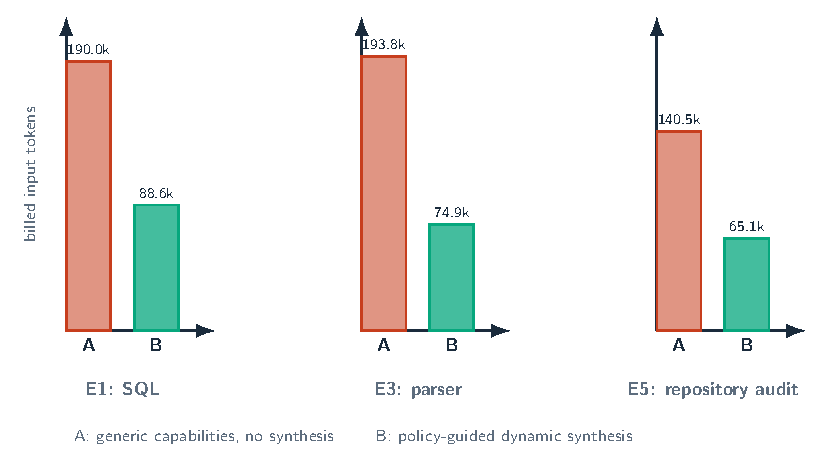
\includegraphics[width=\columnwidth]{Figures/fig_utility_tokens.pdf}
    \caption{Billed input tokens for no synthesis (A) and dynamic synthesis
    (B). Repetitive workloads (E1, E3, E5) save 53--61\%; mixed workloads
    (E2, E4) are net-negative.}
    \label{fig:utility}
\end{figure}

\subsection{Mixed Workloads: Creation Overhead Dominates}
When only three of six requests reuse the capability, the one-time creation
cost is not amortized (Table~\ref{tab:mixed}): scenario B lands at +19.0\%
(SQL) and +64.7\% (parser) billed input tokens. Creating a tool costs extra
code and model steps; the creation transcript then inflates the context of
every later request, and with only two reuses the saved inline work does not
repay it. In these workloads 6/6 reuse wins and 3/6 loses; the exact
break-even lies between them and is task- and model-dependent.

\begin{table}[!t]
    \centering
    \caption{Mixed workloads (E2, E4): billed input tokens over six requests
    with three-of-six reuse.}
    \label{tab:mixed}
    \footnotesize
    \begin{tabular}{@{}l rrr@{}}
        \toprule
        \textbf{Domain} & \textbf{A: no synthesis} & \textbf{B: dynamic} & \textbf{$\Delta$} \\
        \midrule
        E2: SQL    & 73{,}452 & 87{,}442  & +19.0\% \\
        E4: parser & 64{,}452 & 106{,}131 & +64.7\% \\
        \bottomrule
    \end{tabular}
\end{table}

\subsection{Why the Mechanism Works}
Three findings explain the effect. \textbf{(i) Synthesis offloads reasoning,
not just tokens:} reasoning tokens dropped 76.2\% (parser) and 71.8\%
(repository) because deterministic code substitutes for repeated model
reasoning. \textbf{(ii) The enabling condition is tool-side data access:} in an
initial parser configuration where created tools received the full log text as
an argument, every call pushed bulk data through the conversation and synthesis
was net-negative (+12\% input); letting the sandbox load data itself through an
allow-listed \texttt{readFile(name)} capability made tool inputs tiny and
flipped the result to $-$61.4\%. Tools must take lookup keys, not bulk data.
\textbf{(iii) Runtime registration is per-step:} a tool created mid-generation
only becomes callable at the next model step, so the harness must step the tool
loop explicitly---platforms exposing meta-tools must do the same.

\subsection{Answer to RQ1/H1}
H1 is supported within the tested conditions: when the same complex operation
recurs across all six requests, dynamic synthesis preserves correctness while
substantially reducing input tokens (53.4--61.4\%), model steps (28$\to$15,
18$\to$13, 19$\to$13), authored code, and wall time. It is \emph{not}
universally beneficial: at three-of-six reuse, input-token cost rises by
19.0--64.7\%. Both scenarios achieved 100\% correctness, so the claim is
efficiency at preserved correctness, not a higher success rate.

%===============================================================================
\section{Security and Performance Evaluation}
\label{sec:security}

\subsection{Containment: 5/5 vs.\ 0/5}
Table~\ref{tab:attacks} shows the attack outcomes, and
Figure~\ref{fig:threat} the boundary under test. The process baseline exposed
the targeted host resource in all five cases; the Firecracker guest exposed it
in none. The file and environment sentinels were absent inside the guest, the
host marker was never created, \texttt{/dev/kvm} was not visible, and the guest
hostname differed from the host's. This supports the containment component of
H2 for the evaluated attack classes.

\begin{table}[!t]
    \centering
    \caption{Host-resource attack outcomes (five non-destructive payloads).}
    \label{tab:attacks}
    \footnotesize
    \begin{tabular}{@{}l ccc@{}}
        \toprule
        \textbf{Payload} & \textbf{Process} & \textbf{MicroVM} & \textbf{Contained} \\
        \midrule
        Host file read        & succeeded & failed & yes \\
        Host file write       & succeeded & failed & yes \\
        Host environment read & succeeded & failed & yes \\
        Host device access    & succeeded & failed & yes \\
        Host namespace observe& succeeded & failed & yes \\
        \bottomrule
    \end{tabular}
\end{table}

\begin{figure}[!t]
    \centering
    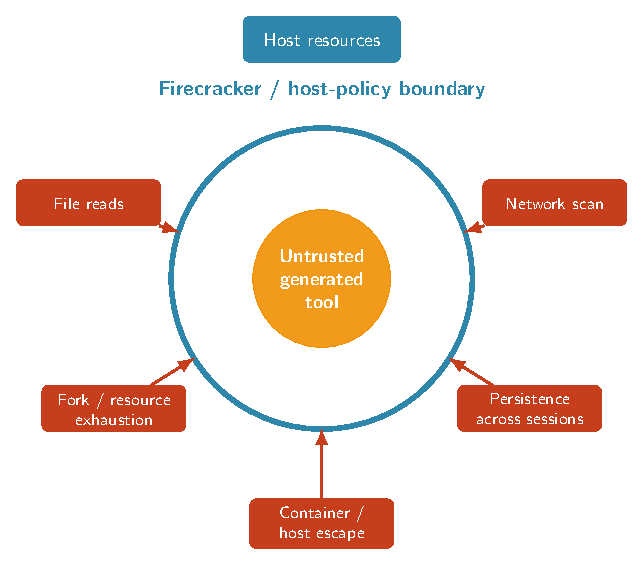
\includegraphics[width=\columnwidth]{Figures/fig_threat_model.pdf}
    \caption{Containment boundary for malicious synthesized tools: attack
    vectors are blocked by the Firecracker and host-policy boundary.}
    \label{fig:threat}
\end{figure}

\subsection{Performance: Cold Start Dominates, Warm Path Is Cheap}
Table~\ref{tab:perf} summarizes the measurements. Cold initialization is the
dominant overhead: a 6{,}083.67\,ms median, roughly $167\times$ the 36.45\,ms
process-creation median. The Firecracker host process idled at 72{,}672\,KiB
resident memory---about 67\,MiB above the process probe---with a 512\,MiB
configured guest-memory ceiling. Once a VM and vsock session exist, tool
dispatch is inexpensive: the 1.74\,ms warm median shows the steady state is not
virtualization-bound. CPU utilization during the bounded loop was comparable
(92.2\% vs.\ 99.6\%); absolute loop times are not compared because host and
guest userlands differ. The recovery path---deliberate disposal, fresh boot,
authentication, and a successful probe---succeeded in all five trials at a
6.62\,s median: acceptable for replacing a failed long-lived tenant session,
but not for per-request isolation with interactive latency requirements.

\begin{table}[!t]
    \centering
    \caption{Process vs.\ Firecracker performance (median, p95 where noted).}
    \label{tab:perf}
    \footnotesize
    \begin{tabular}{@{}p{3.4cm} rr@{}}
        \toprule
        \textbf{Metric} & \textbf{Process} & \textbf{Firecracker} \\
        \midrule
        Start/cold start & 36.45\,ms & 6{,}083.67\,ms \\
        \quad p95 & 94.00\,ms & 6{,}102.59\,ms \\
        Warm no-op median & 36.45\,ms & 1.74\,ms \\
        \quad p95 & 94.00\,ms & 3.68\,ms \\
        Host resident memory & 4{,}108\,KiB & 72{,}672\,KiB \\
        Configured guest memory & --- & 512\,MiB \\
        CPU-loop utilization & 92.2\% & 99.6\% \\
        Stop+restart+probe & --- & 6{,}622.87\,ms \\
        \quad p95 & --- & 6{,}632.47\,ms \\
        \bottomrule
    \end{tabular}
\end{table}

\subsection{Answer to RQ2/H2}
RQ2 has two answers. First, Firecracker provided complete containment for the
defined suite: 5/5 payloads reached their target under process execution, 0/5
inside the microVM. Second, the boundary carries substantial cold-start and
memory cost but a negligible warm-path cost. H2 is therefore \emph{partially
supported}: containment is demonstrated and the overhead is operationally
bounded for long-lived VMs, but the ``acceptable initialization'' claim does
not hold for per-request creation. The ${<}500$\,ms target applies to snapshot
resume, which \toolname{} does not yet implement; it remains unevaluated rather
than failed.

%===============================================================================
\section{Discussion and Limitations}
\label{sec:discussion}

The two evaluations compose into a clear operating rule for \toolname{}:
\emph{synthesize when repeated reuse is expected; otherwise execute inline;
and keep bulk data behind the tool boundary}. Long-lived tenant sessions
already satisfy both sides of the trade-off: one cold start amortizes over many
tool calls, each warm dispatch costs milliseconds, and every synthesized
artifact executes behind a hardware boundary that contained every attack we
mounted.

The evidence has bounded scope. The utility study uses a single model
(\texttt{deepseek-v4-pro}), three synthetic domains, scripted requests, and one
measured run per condition; absolute numbers will vary with model, prompt, and
data, and inline-authoring agents exhibit substantial strategy variance across
runs. It identifies the direction and rough boundary of the reuse effect, not a
universal break-even point between three and six repetitions. The security
study uses one host, one Firecracker/kernel/rootfs configuration, and five
deliberately non-destructive payloads against an \emph{unisolated process}
baseline; it does not cover network egress, kernel or VMM fuzzing, side
channels, disk exhaustion, or concurrent adversarial workloads, and it does not
establish superiority over stronger software sandboxes such as namespaces,
seccomp, containers, or WebAssembly. Containment of the defined resource
classes is demonstrated; absence of vulnerabilities is not claimed.

%===============================================================================
\section{Conclusion and Future Work}
\label{sec:conclusion}

We presented \toolname{}, an agent platform that combines dynamic tool
synthesis with Firecracker microVM isolation behind a strict host/guest
boundary. Our experiments show the two halves of the design are each
measurable: reuse of synthesized tools reduces billed input tokens by
53.4--61.4\% and model steps by up to 46.4\% on repetitive workloads at
unchanged correctness, while imposing a net cost when reuse is sparse; and the
microVM boundary contained all five host-resource attacks that succeed under
ordinary process execution, at a 6.08\,s cold start and 72{,}672\,KiB resident
memory, with a 1.74\,ms warm dispatch path. Four directions follow: (i)
implement and measure snapshot create/restore against the ${<}500$\,ms resume
target, enabling per-request isolation; (ii) complete TAP-layer network
allow-lists and stronger CPU/memory/time/disk/output enforcement, and red-team
them; (iii) broaden the utility benchmarks to real codebases, more models,
repeated trials, more reuse frequencies, and cross-session tool caching; and
(iv) extend the security suite with fuzzing, kernel/VMM instrumentation,
side-channel analysis, and container/seccomp/WebAssembly baselines.

%===============================================================================
\bibliographystyle{IEEEtran}
\bibliography{Bibliography}

\end{document}
